\documentclass[border=6pt]{standalone}
\usepackage{tikz}
\usetikzlibrary{arrows.meta,positioning,fit,calc}
\definecolor{fg}{HTML}{3B3220}
\definecolor{fgbody}{HTML}{544736}
\definecolor{stroke}{HTML}{7A5A10}
\definecolor{surf}{HTML}{FAF6EE}
\definecolor{surfemph}{HTML}{F2E9D4}
\definecolor{surfact}{HTML}{F6E7E0}
\definecolor{bdim}{HTML}{CFC6B2}
\definecolor{bemph}{HTML}{7A5A10}
\definecolor{bact}{HTML}{8F1D1D}
\begin{document}
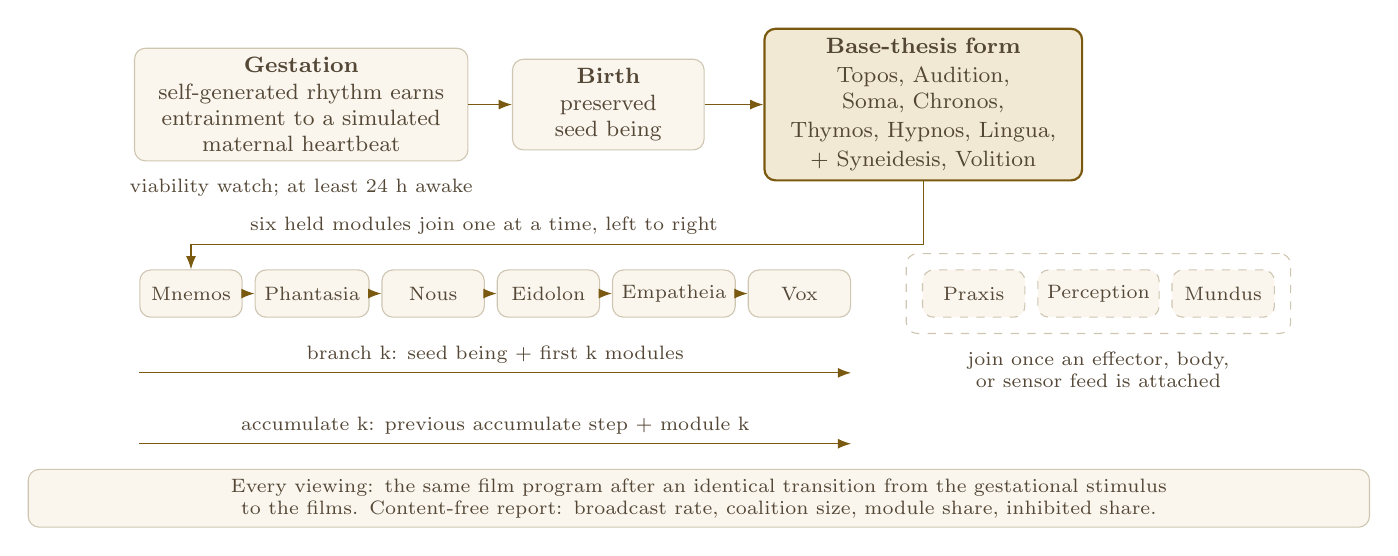
\begin{tikzpicture}[
  font=\footnotesize,>=Latex,
  every node/.append style={text=fgbody, execute at begin node={\hyphenpenalty=10000\exhyphenpenalty=10000}},
  mod/.style={draw=bdim, rounded corners, fill=surf, align=center, font=\footnotesize},
  work/.style={draw=bemph, thick, rounded corners, fill=surfemph, align=center},
  lbl/.style={font=\footnotesize, text=fgbody, align=center},
  held/.style={mod, minimum width=13mm, minimum height=6mm, font=\scriptsize},
]

% Stage 1
\node[mod, text width=40mm] (stage1) at (0,2)
  {\textbf{Gestation}\\self-generated rhythm earns\\entrainment to a simulated\\maternal heartbeat};
\node[lbl, font=\scriptsize, below=1mm of stage1]
  {viability watch; at least 24 h awake};

% Stage 2
\node[mod, text width=22mm] (stage2) at (3.9,2)
  {\textbf{Birth}\\preserved seed being};
\draw[->, draw=stroke] (stage1.east) -- (stage2.west);

% Stage 3
\node[work, text width=38mm] (stage3) at (7.9,2)
  {\textbf{Base-thesis form}\\[1pt]
   Topos, Audition, Soma, Chronos,\\[1pt]
   Thymos, Hypnos, Lingua,\\[1pt]
   + Syneidesis, Volition};
\draw[->, draw=stroke] (stage2.east) -- (stage3.west);

% Held modules
\node[held] (m1) at (-1.4,-0.4) {Mnemos};
\node[held, right=1.5mm of m1] (m2) {Phantasia};
\node[held, right=1.5mm of m2] (m3) {Nous};
\node[held, right=1.5mm of m3] (m4) {Eidolon};
\node[held, right=1.5mm of m4] (m5) {Empatheia};
\node[held, right=1.5mm of m5] (m6) {Vox};
\node[held, dashed, right=9mm of m6] (m7) {Praxis};
\node[held, dashed, right=1.5mm of m7] (m8) {Perception};
\node[held, dashed, right=1.5mm of m8] (m9) {Mundus};
\node[draw=bdim, dashed, rounded corners, fit=(m7)(m8)(m9), inner sep=2mm] (later) {};
\node[lbl, font=\scriptsize, text width=48mm, below=1mm of later] {join once an effector, body, or sensor feed is attached};

\draw[->, draw=stroke] (stage3.south) -- ++(0,-0.8) -| node[pos=0.3, above, font=\scriptsize] {six held modules join one at a time, left to right} (m1.north);

\foreach \i/\j in {1/2,2/3,3/4,4/5,5/6}{
  \draw[->, draw=stroke] (m\i.east) -- (m\j.west);
}

% Recurrence arrows
\draw[->, draw=stroke, thin]
  ($(m1.south west)+(0,-0.7)$) -- ($(m6.south east)+(0,-0.7)$)
  node[pos=0.5, above, font=\scriptsize] {branch k: seed being + first k modules};
\draw[->, draw=stroke, thin]
  ($(m1.south west)+(0,-1.6)$) -- ($(m6.south east)+(0,-1.6)$)
  node[pos=0.5, above, font=\scriptsize] {accumulate k: previous accumulate step + module k};

% Footer
\node[mod, text width=168mm, font=\scriptsize] at (5.05,-3.0)
  {Every viewing: the same film program after an identical transition from the gestational stimulus to the films.
   Content-free report: broadcast rate, coalition size, module share, inhibited share.};

\end{tikzpicture}
\end{document}
